\documentclass[12pt,epsf]{report}
\usepackage[left=2cm, right=2cm, bottom=2cm,top=2cm]{geometry}
\usepackage[myheadings]{fullpage}
\usepackage{fancyhdr}
\usepackage{lastpage}
\usepackage{graphicx, wrapfig, subcaption, setspace, booktabs}
\usepackage[T1]{fontenc}
\usepackage[font=small, labelfont=bf]{caption}
\usepackage{fourier}
\usepackage[protrusion=true, expansion=true]{microtype}
\usepackage[english]{babel}
\usepackage{sectsty}
\usepackage[section]{placeins}
\graphicspath{{plot/}}

\newcommand{\HRule}[1]{\rule{\linewidth}{#1}}
\onehalfspacing
\setcounter{tocdepth}{5}
\setcounter{secnumdepth}{5}
\usepackage{verbatim}
%-------------------------------------------------------------------------------
% HEADER & FOOTER
%-------------------------------------------------------------------------------
\pagestyle{fancy}
\fancyhf{}
\setlength\headheight{15pt}
\fancyhead[L]{Group Number 6}
\fancyhead[R]{Statistical Methods in Research}
\fancyfoot[R]{Page \thepage\ of \pageref{LastPage}}
%-------------------------------------------------------------------------------
% TITLE PAGE
%-------------------------------------------------------------------------------

\begin{document}

\title{ \large \textsc{Statistical Methods in Research}
		\\ [2.0cm]
		\HRule{1pt} \\
		\LARGE \textbf{{Analysis of How Stress Patterns Define Human Experience and Performance in Dexterous Tasks}}
		\HRule{1pt} \\ [0.5cm]
		\normalsize \today \vspace*{5\baselineskip}}

\date{}

\author{
		Suchismitha Vedala \\ 
		Lavanya Rao \\
		Yashwanth Reddy Venati }

\maketitle
\tableofcontents
\newpage

%-------------------------------------------------------------------------------
% Section title formatting
\sectionfont{\scshape}
%-------------------------------------------------------------------------------

%-------------------------------------------------------------------------------
% BODY
%-------------------------------------------------------------------------------

\section*{Introduction}
\addcontentsline{toc}{section}{Introduction}
{The Microsurgery performance data represents the performance of 22 medical students in microsurgery activities. The 22 medical students or subjects in our analysis, participated in a longitudinal study regarding the relationship of sympathetic arousal and skill in learning micro-surgical tasks. The subjects had to pay five visits which we regard as sessions, lasting one hour each, in order to practice micro-surgical cutting and suturing in an inanimate simulator.A pre and post study questionnaire was also given to be completed by the subjects to know a little about their biography and anxiety.\\
\\
During the main part of each session, the subjects underwent the following treatments:\\
1.Baseline: The subjects were relaxing for 5 min, listening to spa music. They were facially recorded by a thermal and visual camera.\\
2.Cutting: The subjects had to precision cutting in the inanimate simulator. They were facially recorded by a thermal and visual camera.\\
3.Suturing: The subjects had to perform suturing in the inanimate simulator. They were facially recorded by a thermal and visual camera.\\
\\
Explicit accuracy scores per task is provided in the data. Hence, the cutting task has its own accuracy scores and so is the case with the suturing task. The perspiration values are recorded in all time frames for all subjects and sessions. The subjects were asked to fill out a  NASA-TLX questionnaire after each task. he NASA-TLX instrument features five subscales measuring different aspects of the subjects' perceptions regarding task difficulty.We perform an analysis with this given data.\\   }

\newpage
\section*{Initial Analysis}
\addcontentsline{toc}{section}{Initial Analysis}
\subsection*{Biographic Data}
\addcontentsline{toc}{subsection}{Biographic Data}
We draw a bar plot to see how gender defines data and histogram to see whether age has any effect on the data.\\
\begin{figure}[!htb]
	\begin{minipage}[c]{0.5\linewidth}
	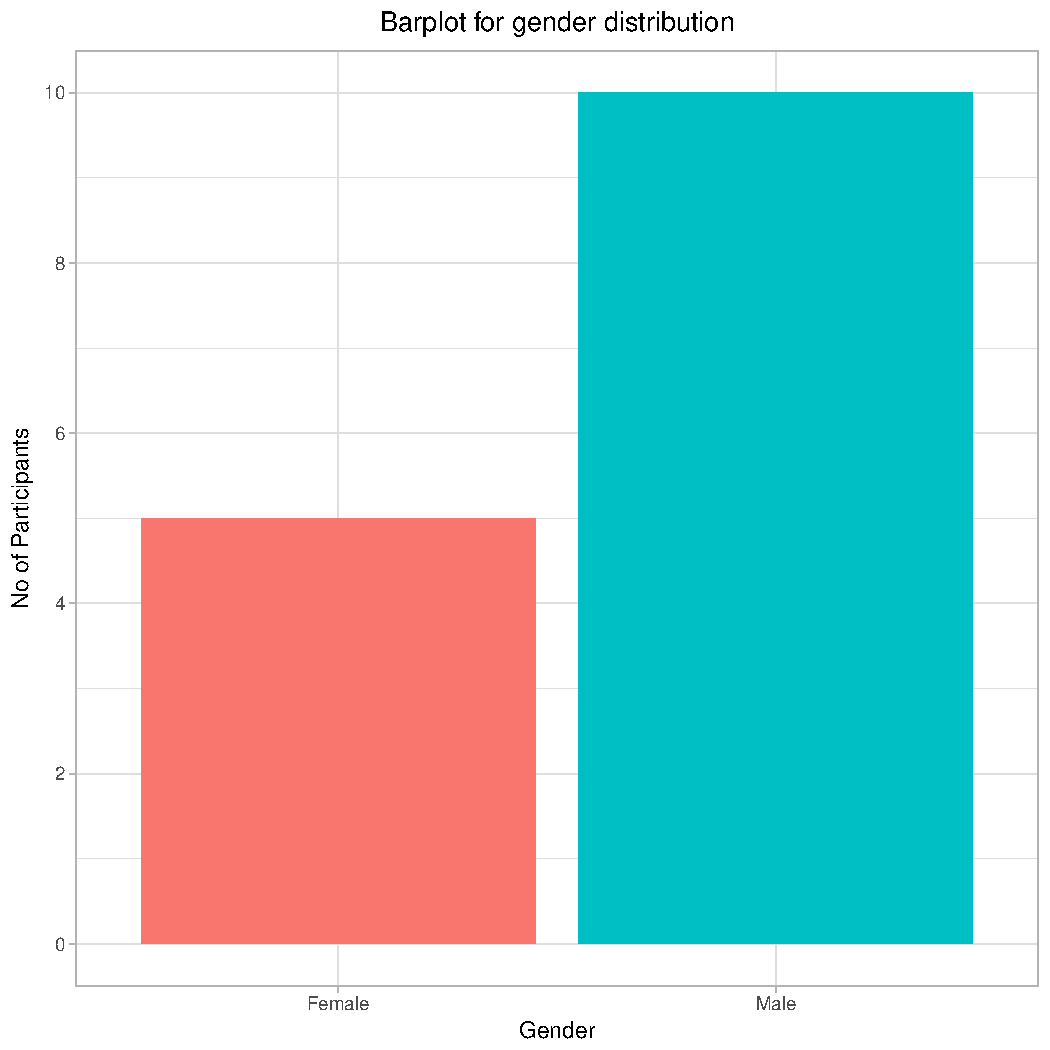
\includegraphics[width=\linewidth]{1_gender.pdf}
	\caption{Barplot of Gender Distribution}
	\end{minipage}
	\hfill
	\begin{minipage}[c]{0.5\linewidth}
	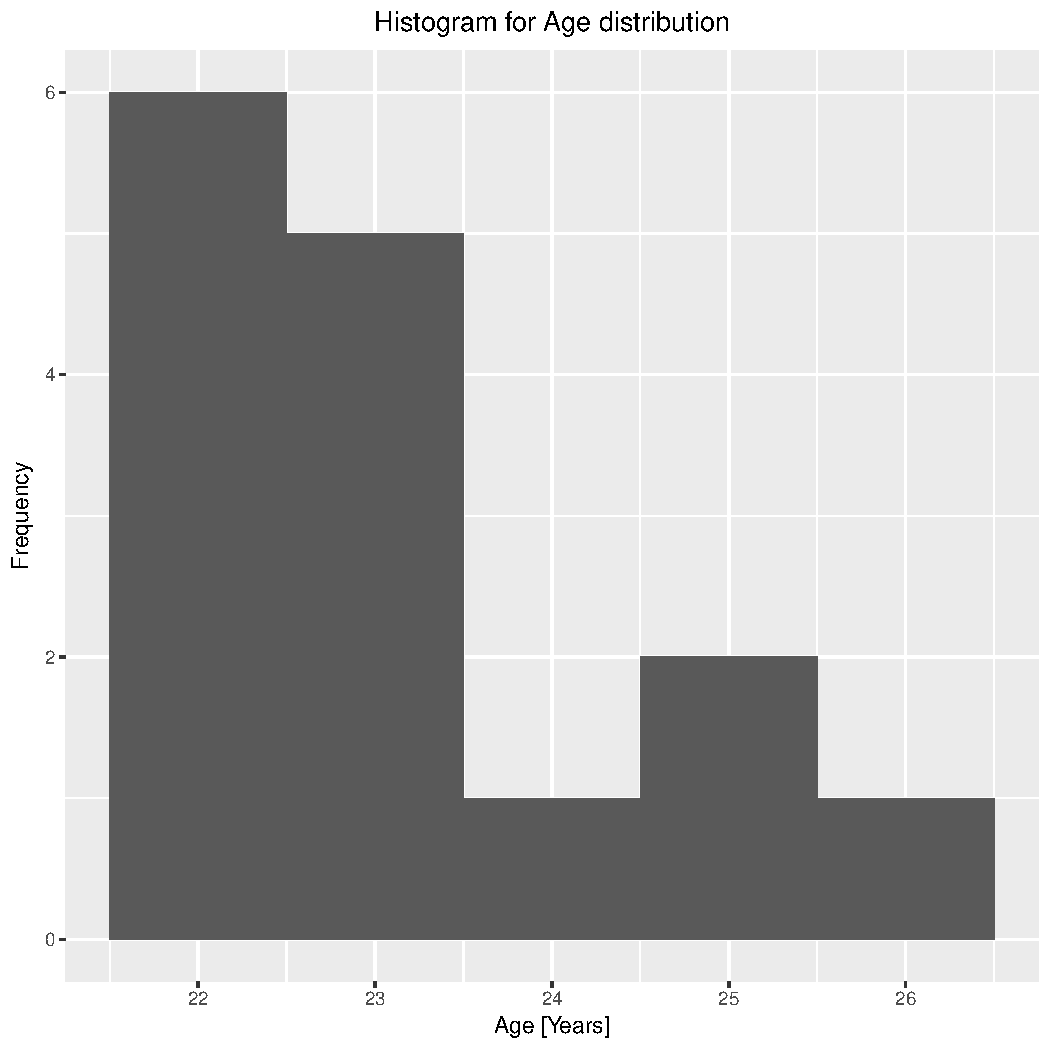
\includegraphics[width=\linewidth]{1_age.pdf}
	\caption{Histogram of age distribution}
	\end{minipage}
\end{figure}

\subsection*{Trait Psychometric Data}
\addcontentsline{toc}{subsection}{Trait Psychometric Data}
We draw the histogram for Trait Anxiety Inventory(TAI) scores\\
\begin{figure}[!htb]
	\centering
	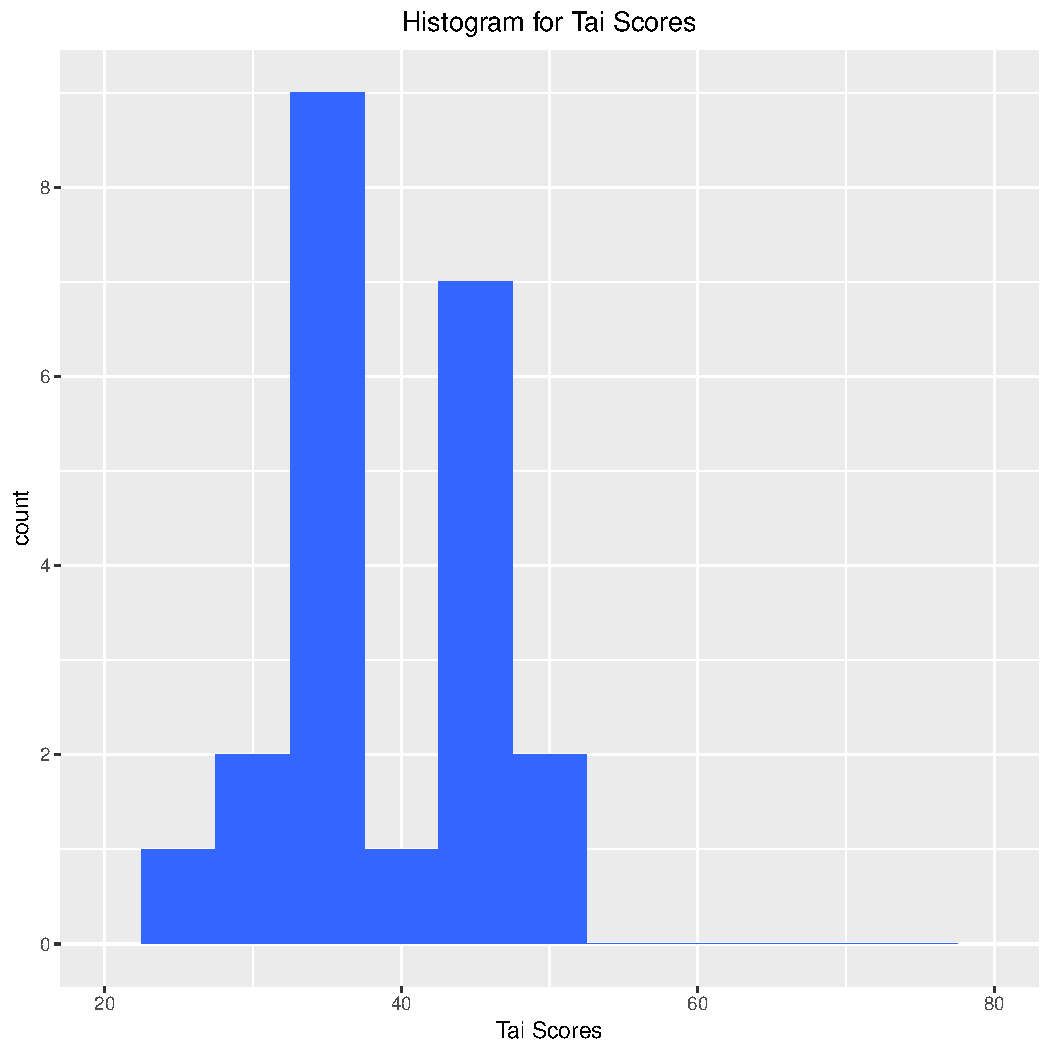
\includegraphics[width=0.5\textwidth]{tai_plot.pdf}
	\caption{Histogram of Tai Scores}
	\centering
\end{figure}
\newpage
\subsection*{State Psychometric Data}
\addcontentsline{toc}{subsection}{State Psychometric Data}
For each subject draw the bar plots for all the NASA-TLX subscales per task. This will give two figures per subject per subscale, one for suturing and one for cutting, where the evolution of the scores from the initial to the final session will be evident. \\
\begin{figure}[!htb]
	\begin{minipage}[c]{0.5\linewidth}
	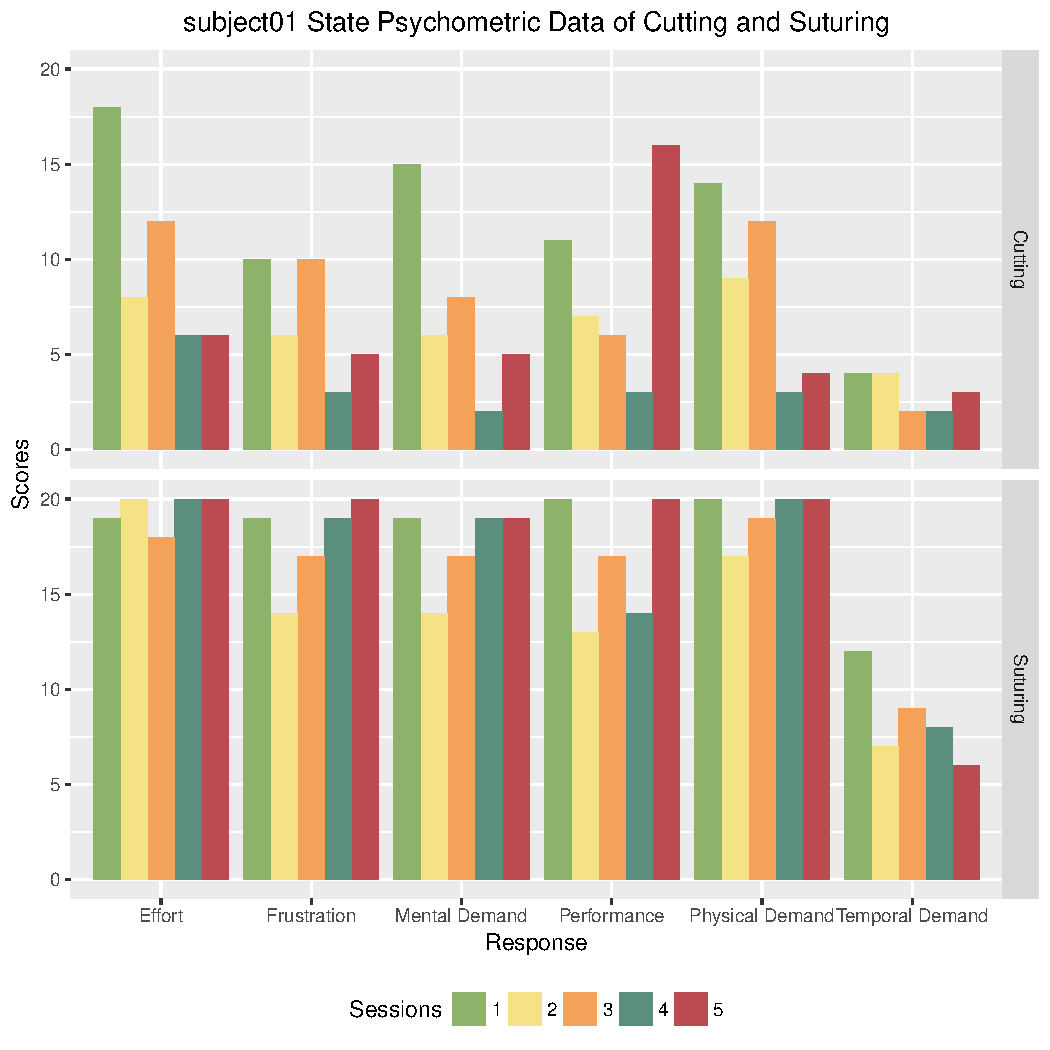
\includegraphics[width=\linewidth]{subject01_State_Psychometric_Data_of_Cutting_and_Suturing.pdf}
	\caption{Subject 1 }
	\end{minipage}
	\hfill
	\begin{minipage}[c]{0.5\linewidth}
	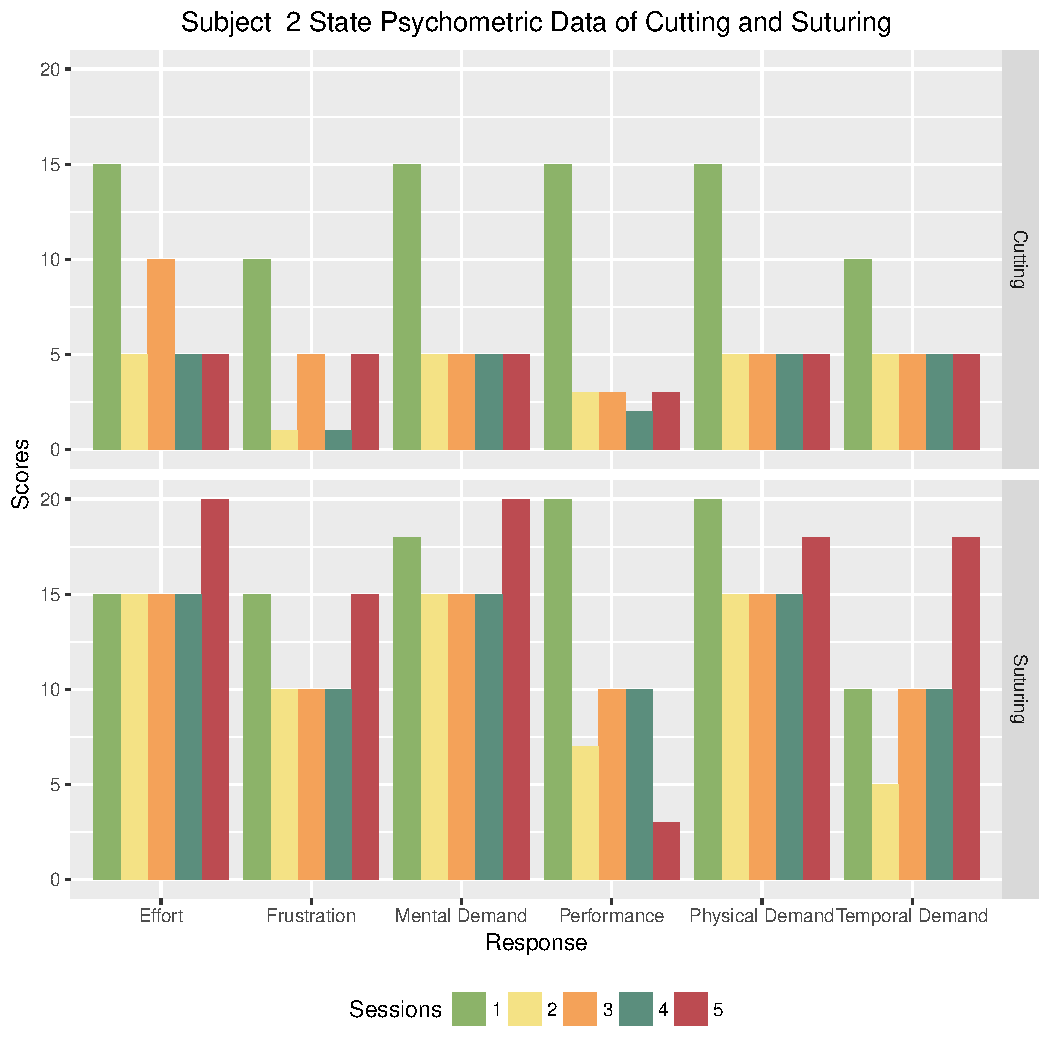
\includegraphics[width=\linewidth]{subject02_State_Psychometric_Data_of_Cutting_and_Suturing.pdf}
	\caption{Subject 2}
	\end{minipage}
\end{figure}

\subsection*{Perinasal Perspiration (Stress) Signal Data}
\addcontentsline{toc}{subsection}{Perinasal Perspiration (Stress) Signal Data}
For each session of each subject  we draw the perspiration values using black for baseline, green for cutting, and red for suturing. 
\begin{figure}[!htb]
	\begin{minipage}[c]{0.5\linewidth}
	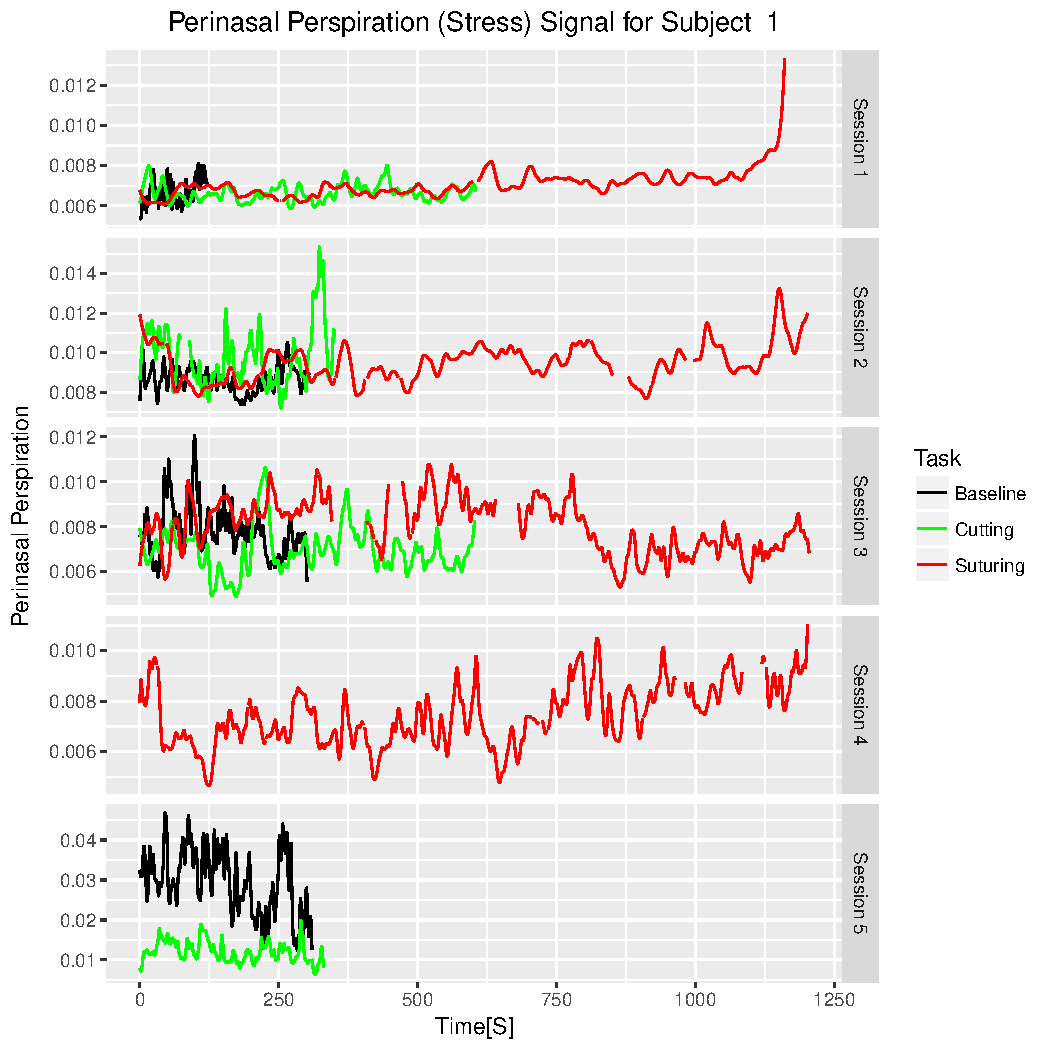
\includegraphics[width=\linewidth]{s1pp.pdf}
	\caption{Subject 1 }
	\end{minipage}
	\hfill
	\begin{minipage}[c]{0.5\linewidth}
	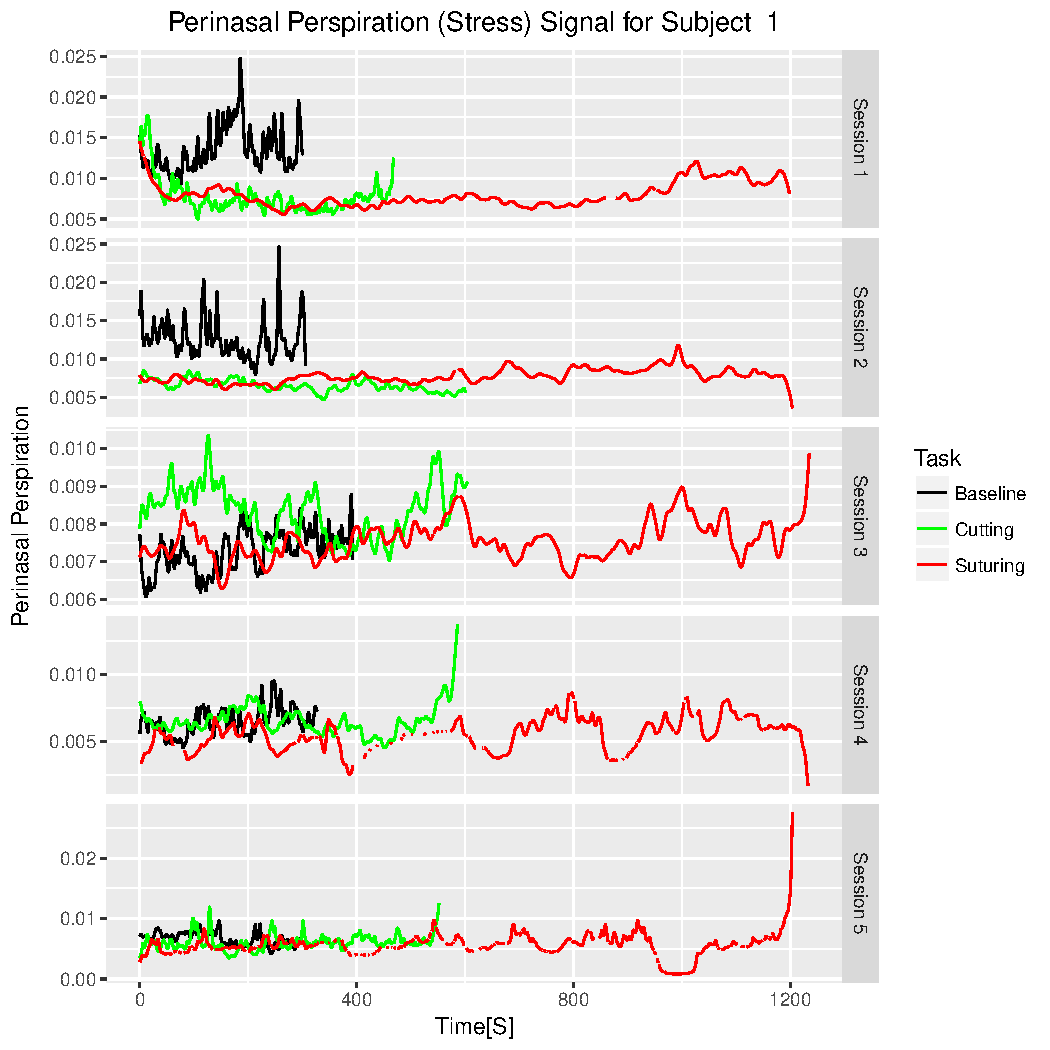
\includegraphics[width=\linewidth]{s2pp.pdf}
	\caption{Subject 2}
	\end{minipage}
\end{figure}
\FloatBarrier
\subsection*{Performance Data}
\addcontentsline{toc}{subsection}{Performance Data}
We draw the accuracy and time bar plots of each subject for each session and each task.\\
\begin{figure}[!htb]
	\centering
	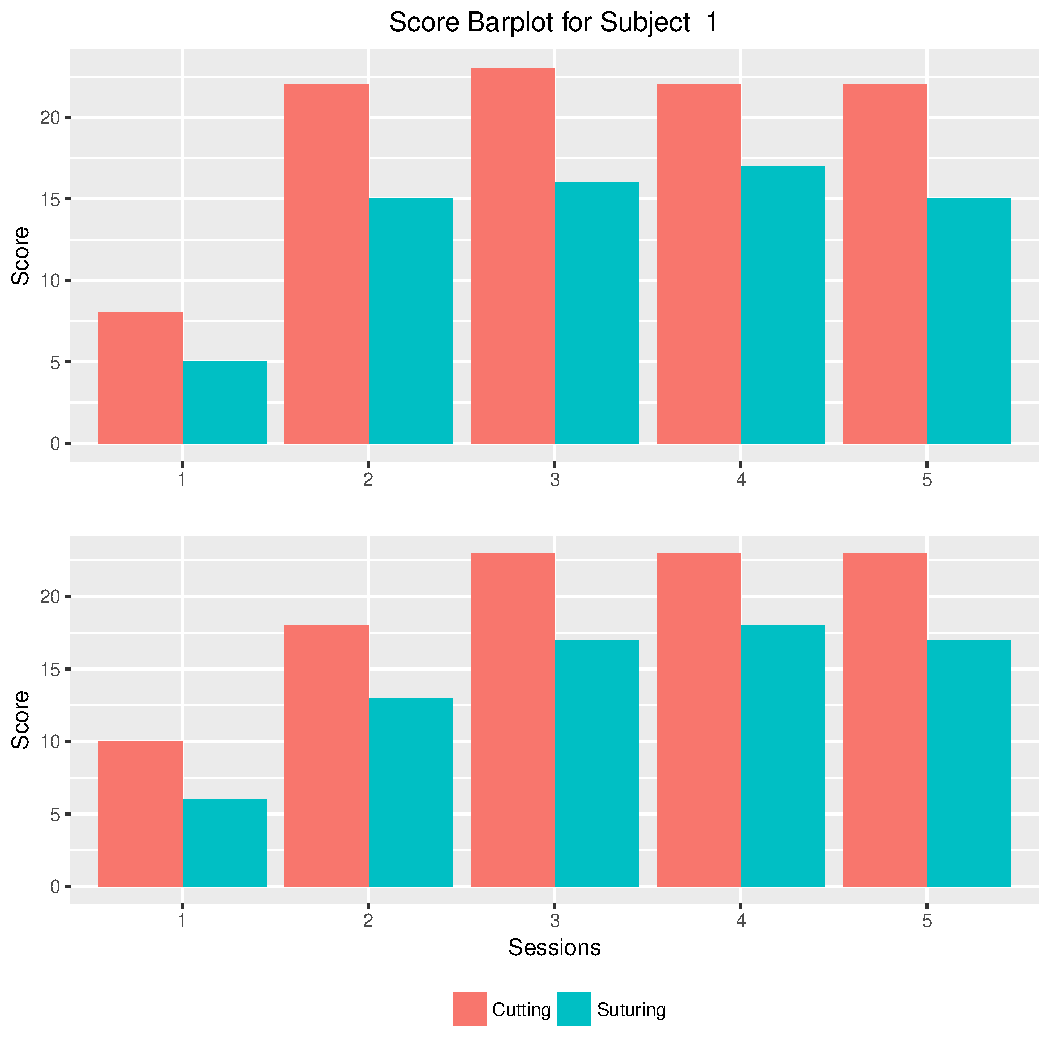
\includegraphics[width=0.5\textwidth]{1Score_barplot.pdf}
	\caption{Subject 1 Score Barplot}
	\centering
\end{figure}
\\
\begin{figure}[!htb]
	\centering
	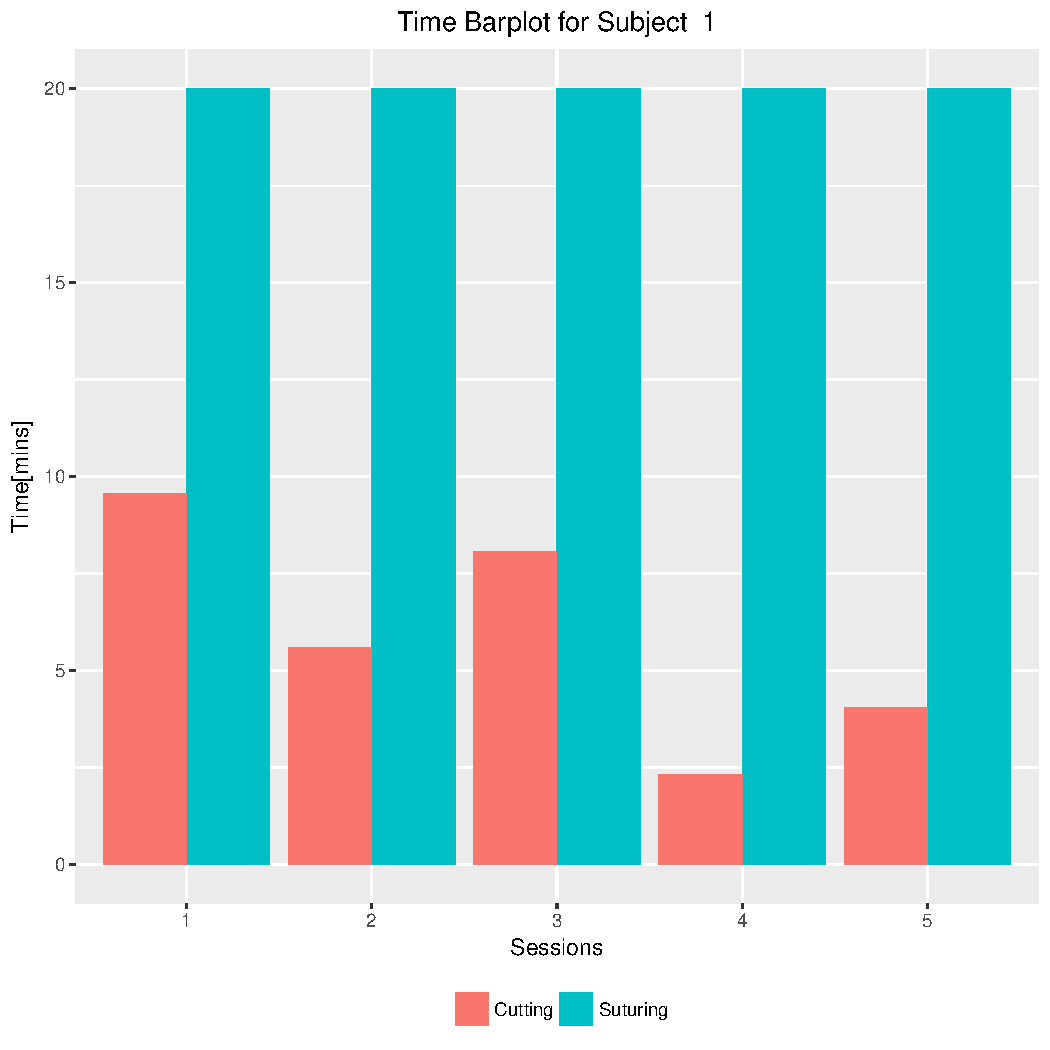
\includegraphics[width=0.5\textwidth]{1Time_barplot.pdf}
	\caption{Subject 1 Time Barplot}
	\centering
\end{figure}\\
\section*{Hypothesis Testing}
We normalize the perspiration values and perform the log of the values for our analysis.\\
\addcontentsline{toc}{section}{Hypothesis Testing}
\subsection*{1. Analysis of effect of each attribute on Score}
\addcontentsline{toc}{subsection}{Analysis of effect of each attribute on Score}
\textbf{Hypothesis}:\\
$Null Hypothesis : H_0 = $ The score obtained does not depend on the demographics of the subject , session , age , year , sex and perspiration.\\
$Alternate Hypothesis : H_1 = $ The score obtained  depends on the demographics of the subject , session , age , year , sex and perspiration.\\
\\
\textbf{Approach:Linear Modelling}:\\
Linear modeling gives the relationship between the dependent and independent variables. 
In our data set we are finding the hypothesis between each attribute such as Age, sex, year and mean perspiration with the scores of scorer.\\
\begin{figure}[!htb]
	\centering
	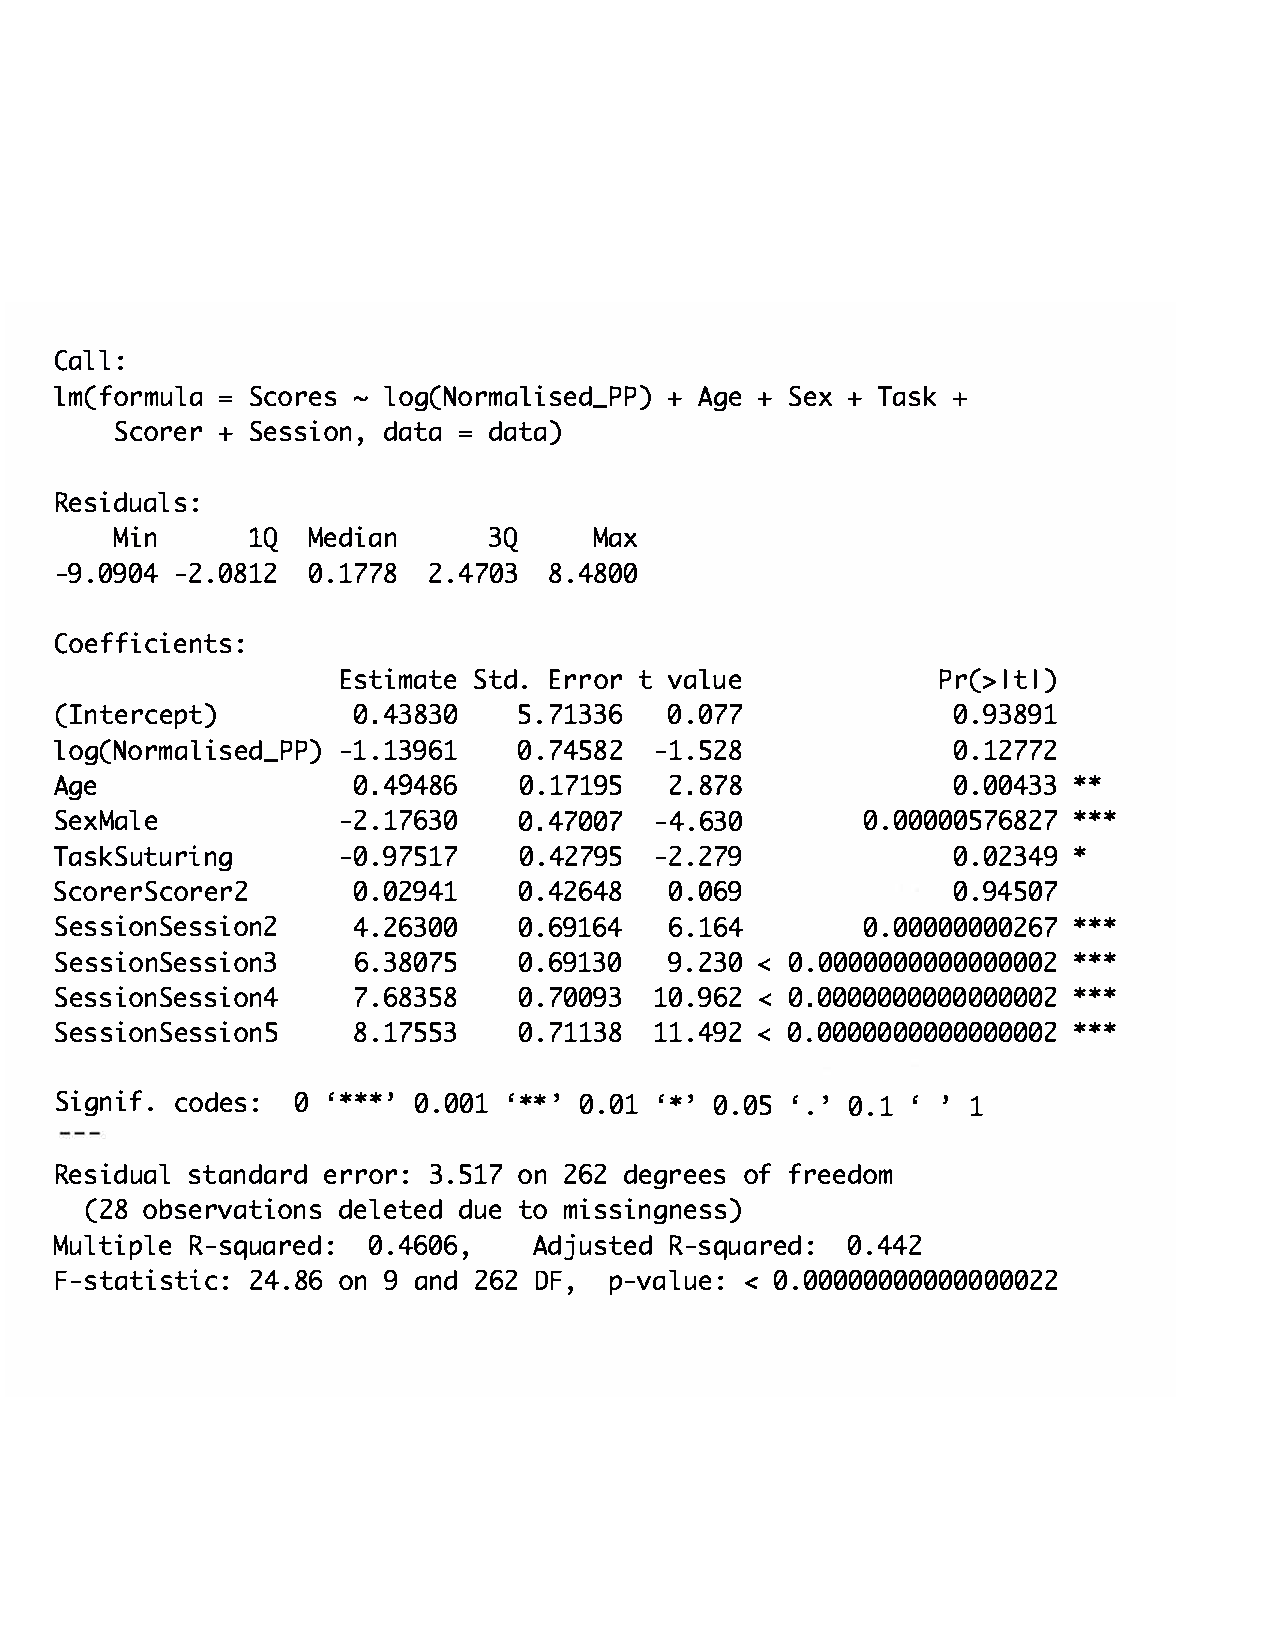
\includegraphics[width=0.5\textwidth]{ScoreSummary.pdf}
	\caption{Linear model of score vs all other attributes}
	\centering
\end{figure}
\\
\begin{figure}[!htb]
	\begin{minipage}[c]{0.5\linewidth}
	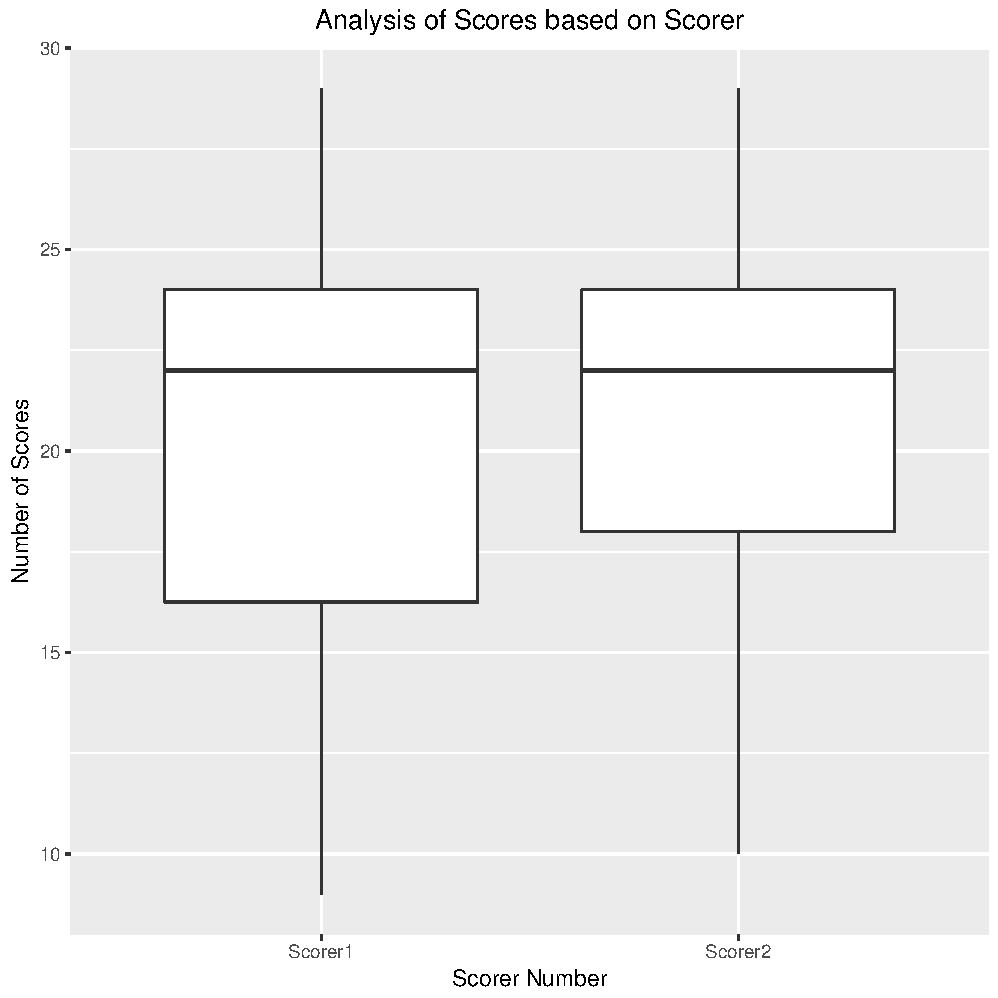
\includegraphics[width=\linewidth]{ScorerVsScore.pdf}
	\caption{Analysis of Scores based on Score }
	\end{minipage}
	\hfill
	\begin{minipage}[c]{0.5\linewidth}
	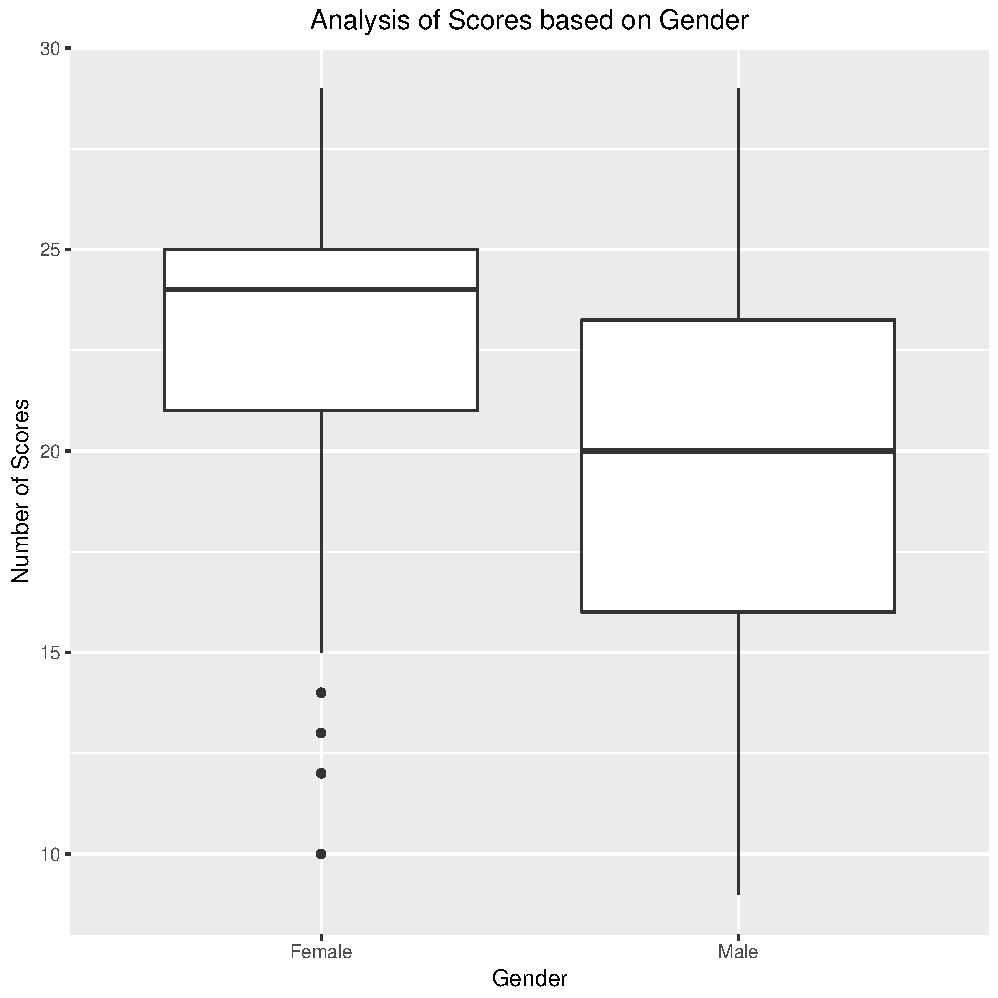
\includegraphics[width=\linewidth]{GenderVsScore.pdf}
	\caption{Analysis of Scores based on Gender}
	\end{minipage}
\end{figure}
\begin{figure}[!htb]
	\begin{minipage}[c]{0.5\linewidth}
	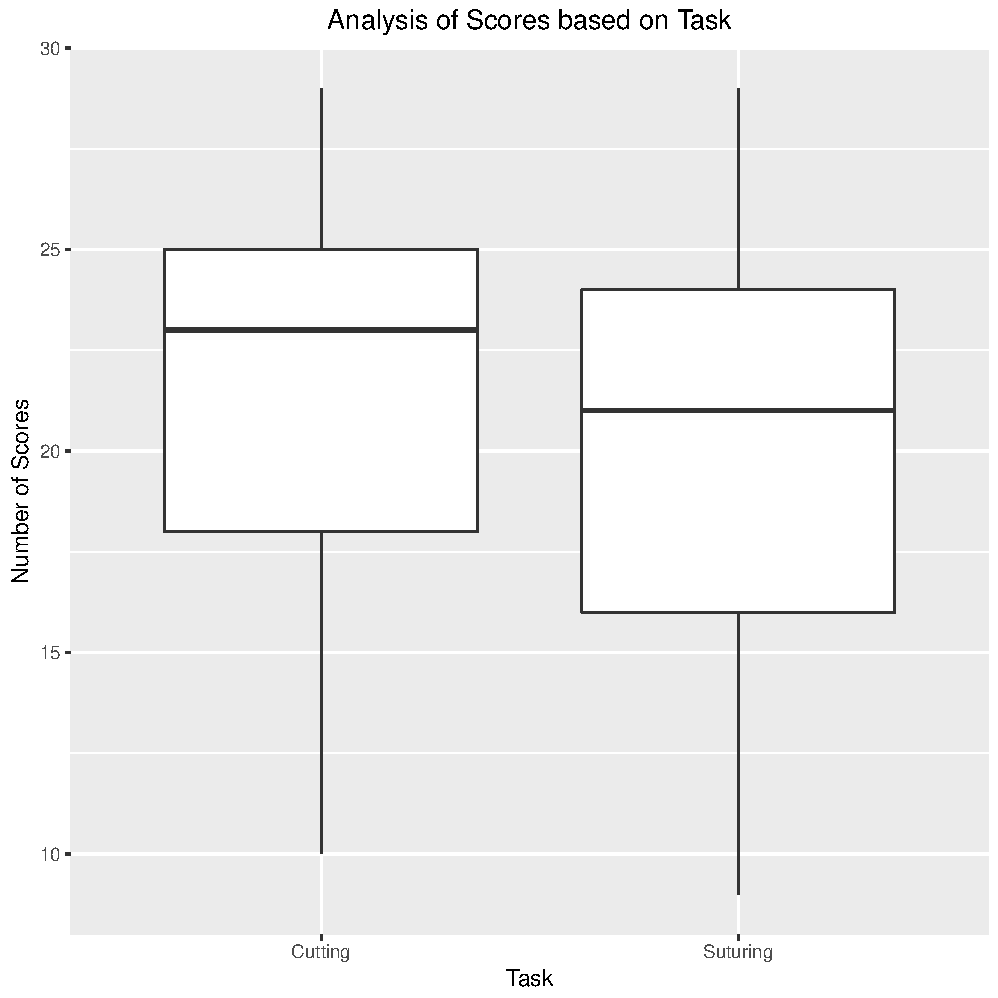
\includegraphics[width=\linewidth]{TaskVsScore.pdf}
	\caption{Analysis of Scores based on Task}
	\end{minipage}
	\hfill
	\begin{minipage}[c]{0.5\linewidth}
	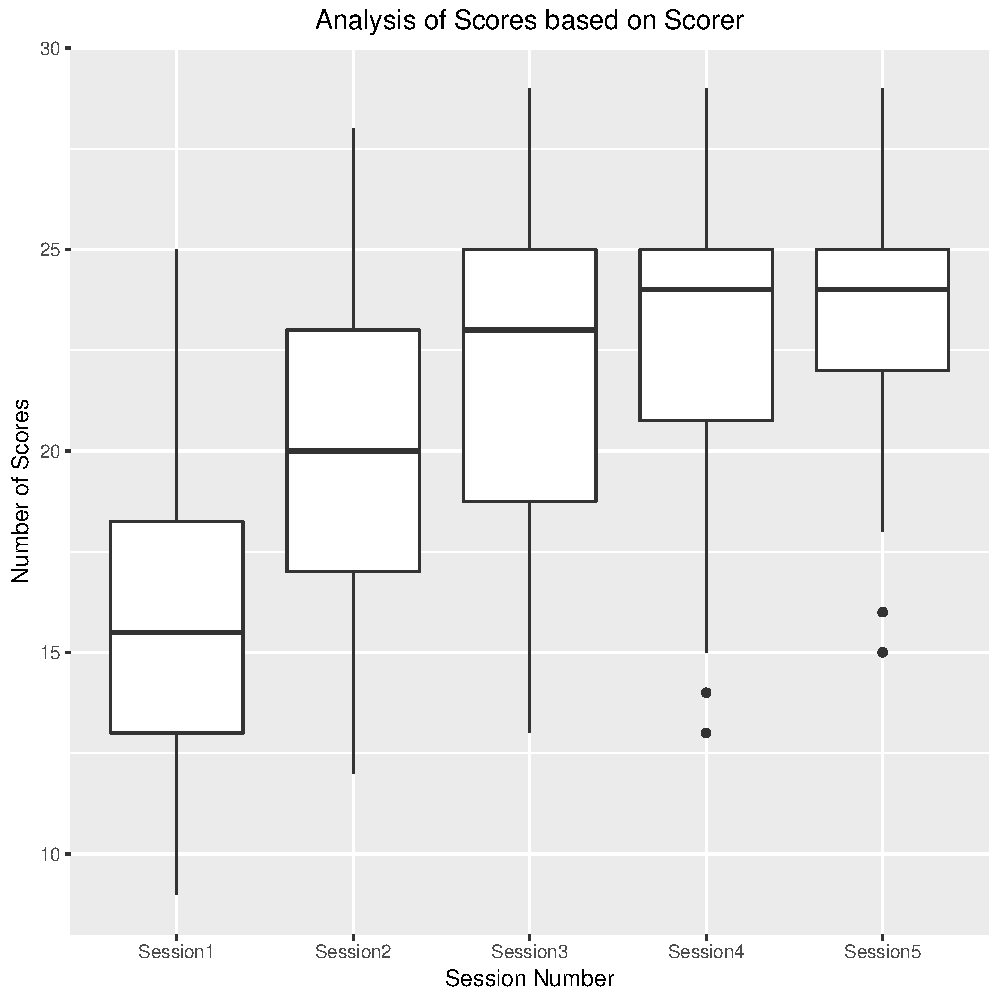
\includegraphics[width=\linewidth]{SessionVsScore.pdf}
	\caption{Analysis of Scores based on Session}
	\end{minipage}
\end{figure}\\
\textbf{Inference}:\\
The above equation informs us that scores will increase by -34.67 for every one percent increase in mean Perspiration value , and score is directly proportional to age which states that the if older age people are hired the score would have increased\\
\\
\FloatBarrier
\subsection*{2. Analysis of effect of each attribute on Time}
\addcontentsline{toc}{subsection}{Analysis of effect of each attribute on Time}
\textbf{Hypothesis}:\\
$Null Hypothesis : H_0 = $ The time taken to do a task is not dependednt of age, session, sex, Perspiration.\\
$Alternate Hypothesis : H_1 = $ he time taken to do a task depends on  age, session, sex, Perspiration.\\
\\
\textbf{Approach:Linear Modelling}:\\
Linear modeling gives the relationship between the dependent and independent variables. 
In our data set we are finding the hypothesis between each attribute such as Age, sex, year and mean perspiration with the time taken to do the task.\\
\begin{figure}[!htb]
	\centering
	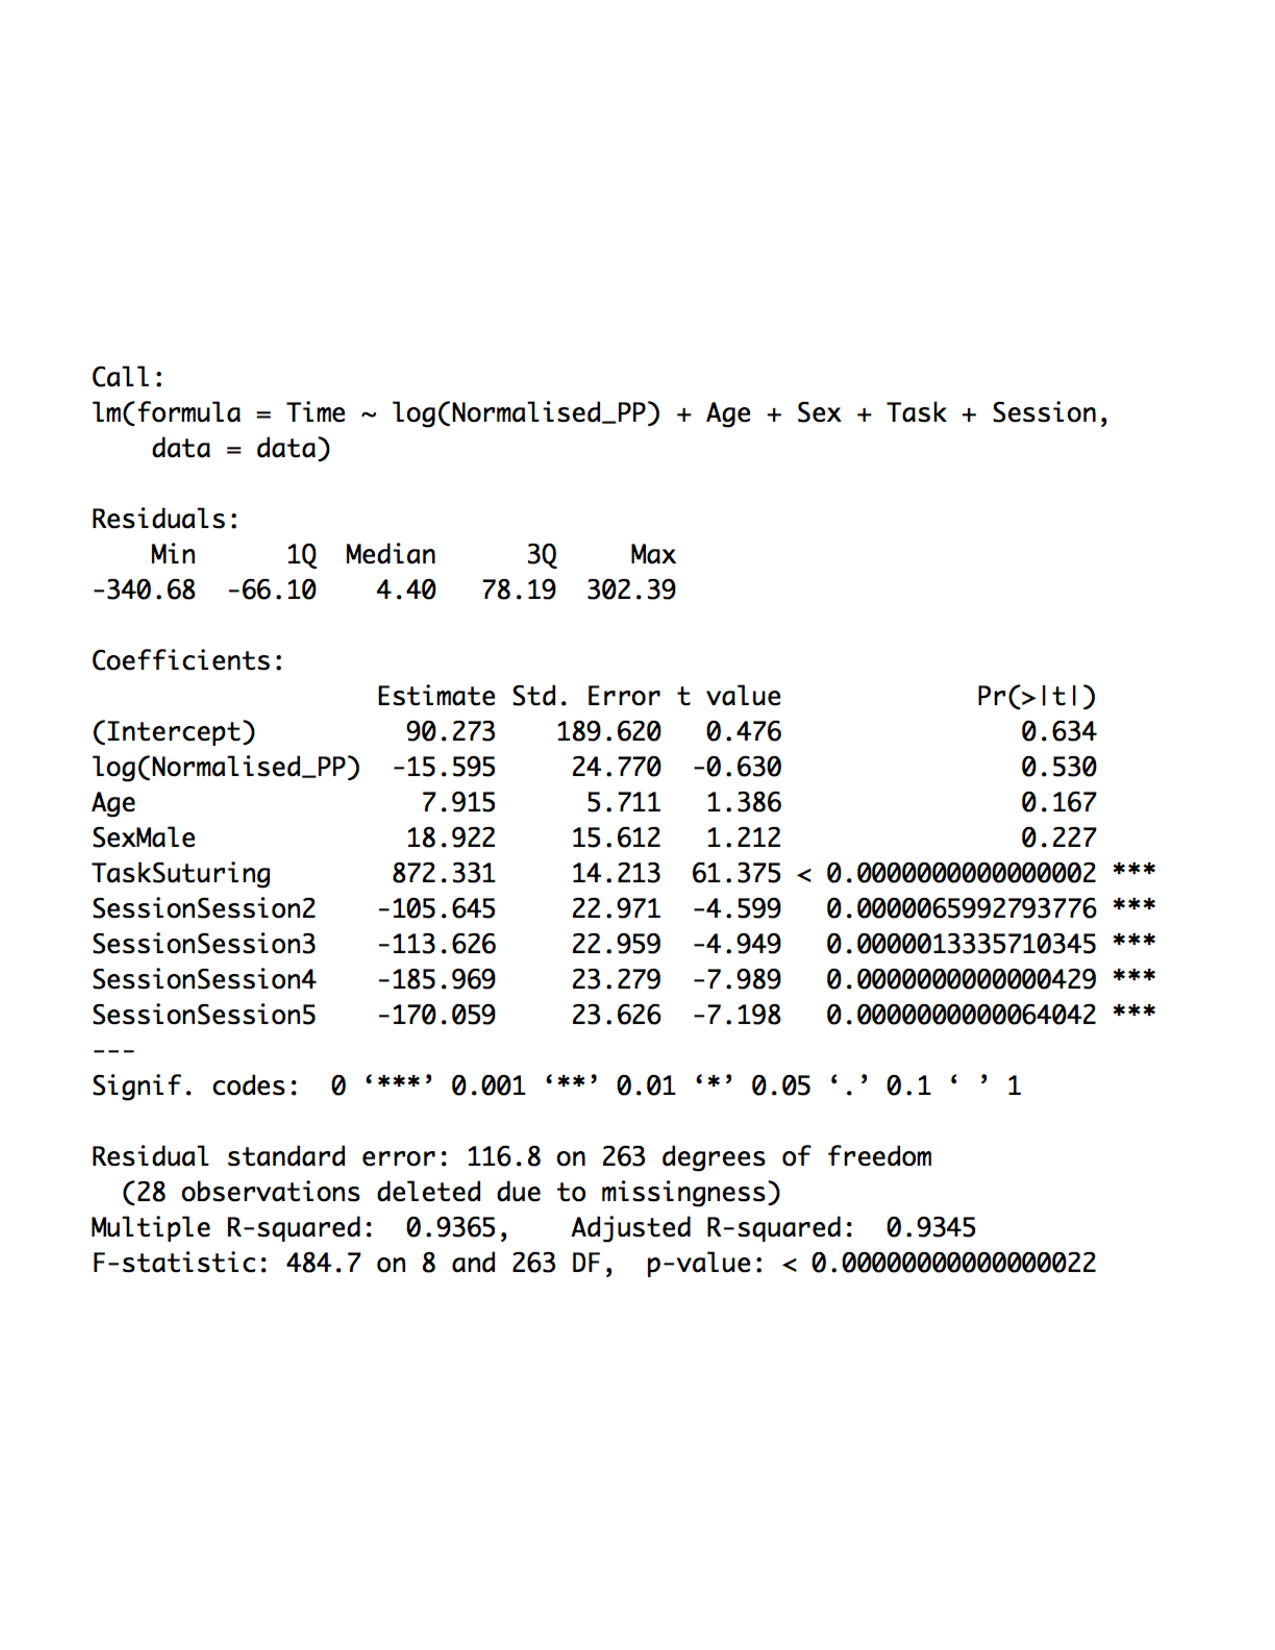
\includegraphics[width=0.5\textwidth]{TimeSummary.pdf}
	\caption{Linear model of Time vs all other attributes}
	\centering
\end{figure}
\\
\begin{figure}[!htb]
	\begin{minipage}[c]{0.5\linewidth}
	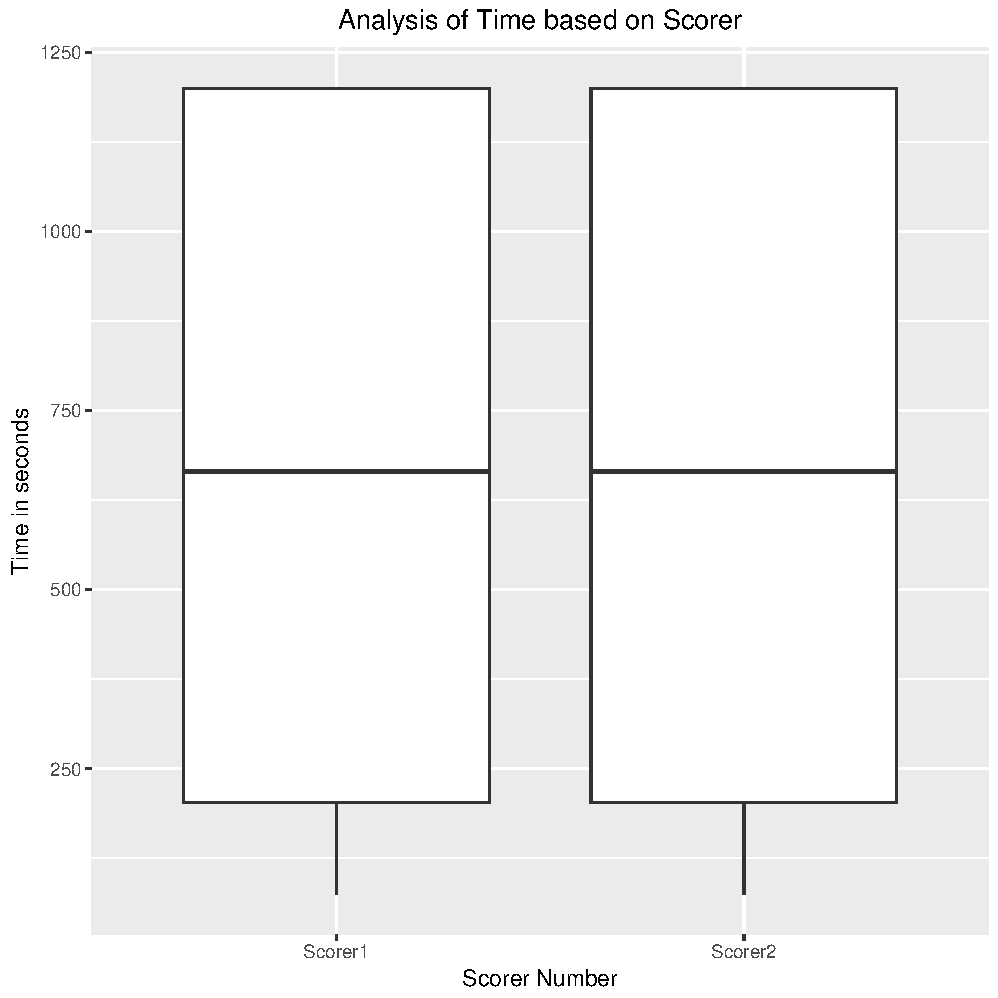
\includegraphics[width=\linewidth]{ScorerVsTime.pdf}
	\caption{Analysis of Time based on Score }
	\end{minipage}
	\hfill
	\begin{minipage}[c]{0.5\linewidth}
	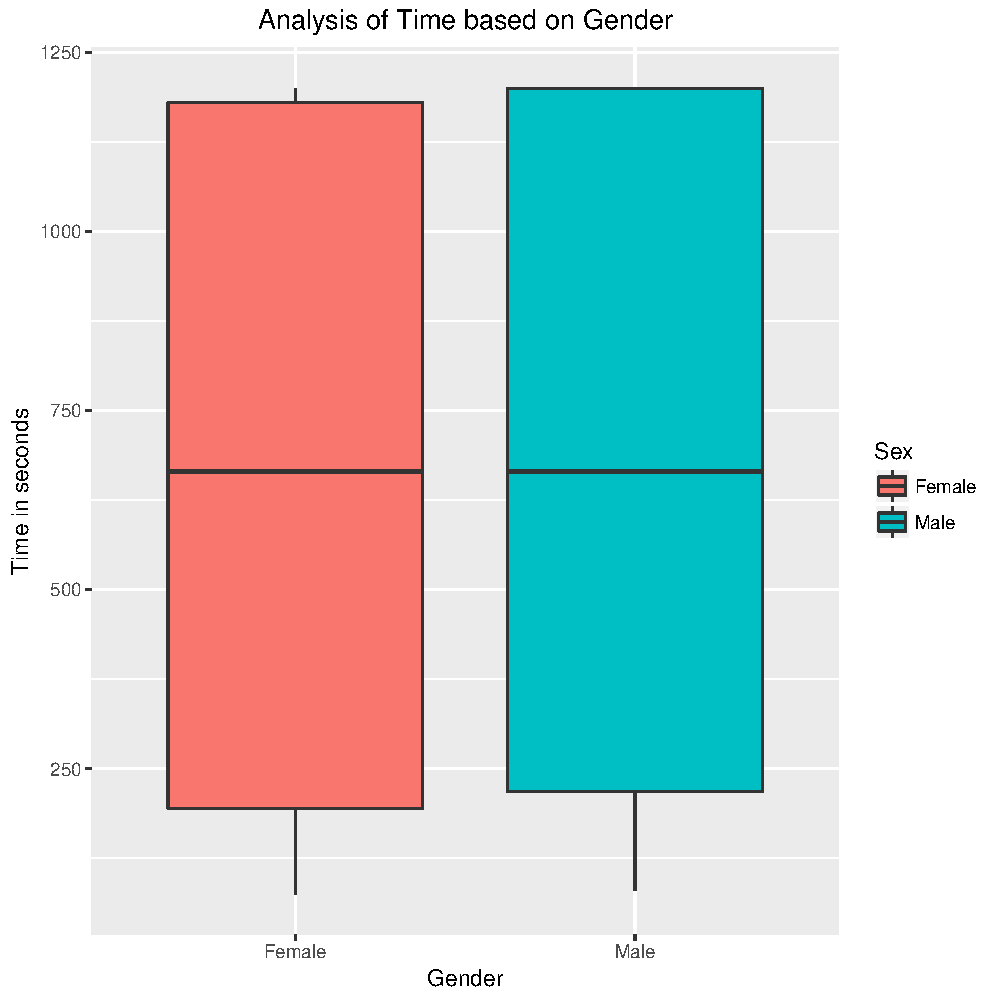
\includegraphics[width=\linewidth]{GenderVsTime.pdf}
	\caption{Analysis of Time based on Gender}
	\end{minipage}
\end{figure}
\begin{figure}[!htb]
	\begin{minipage}[c]{0.5\linewidth}
	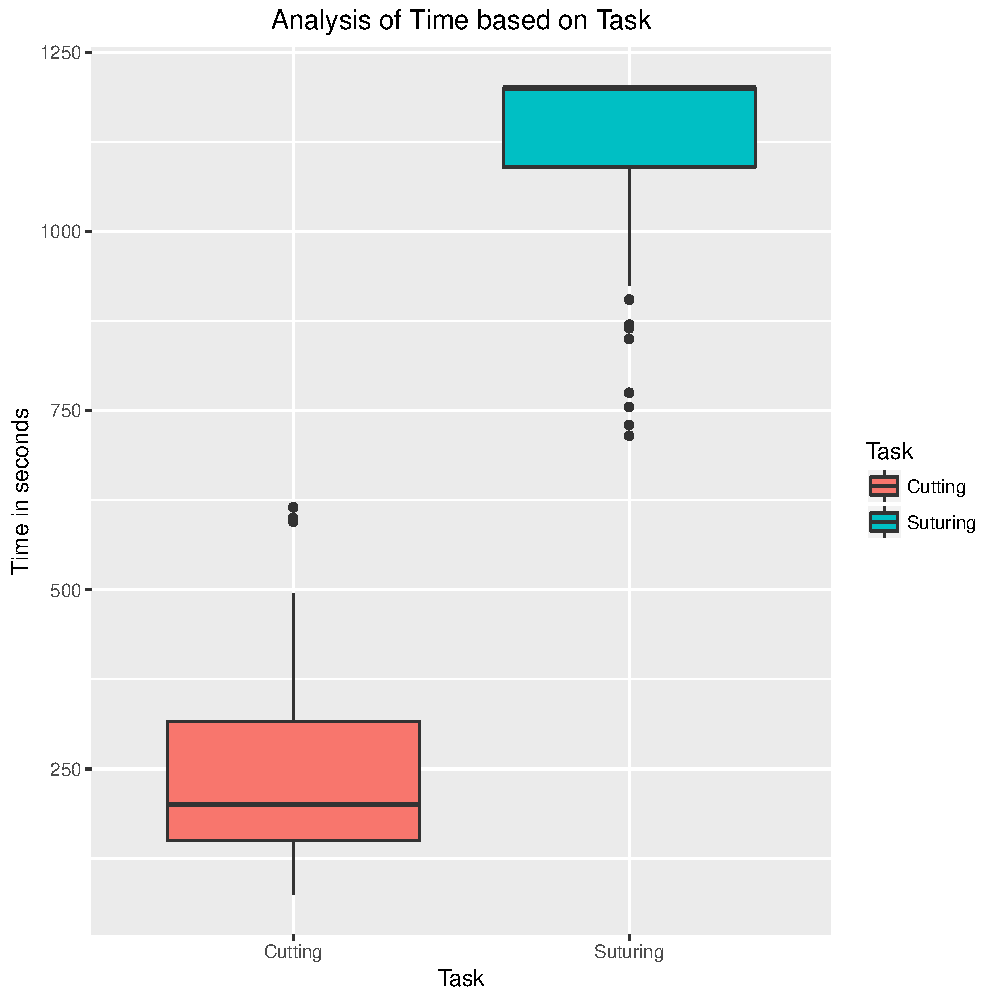
\includegraphics[width=\linewidth]{TaskVsTime.pdf}
	\caption{Analysis of Time based on Task}
	\end{minipage}
	\hfill
	\begin{minipage}[c]{0.5\linewidth}
	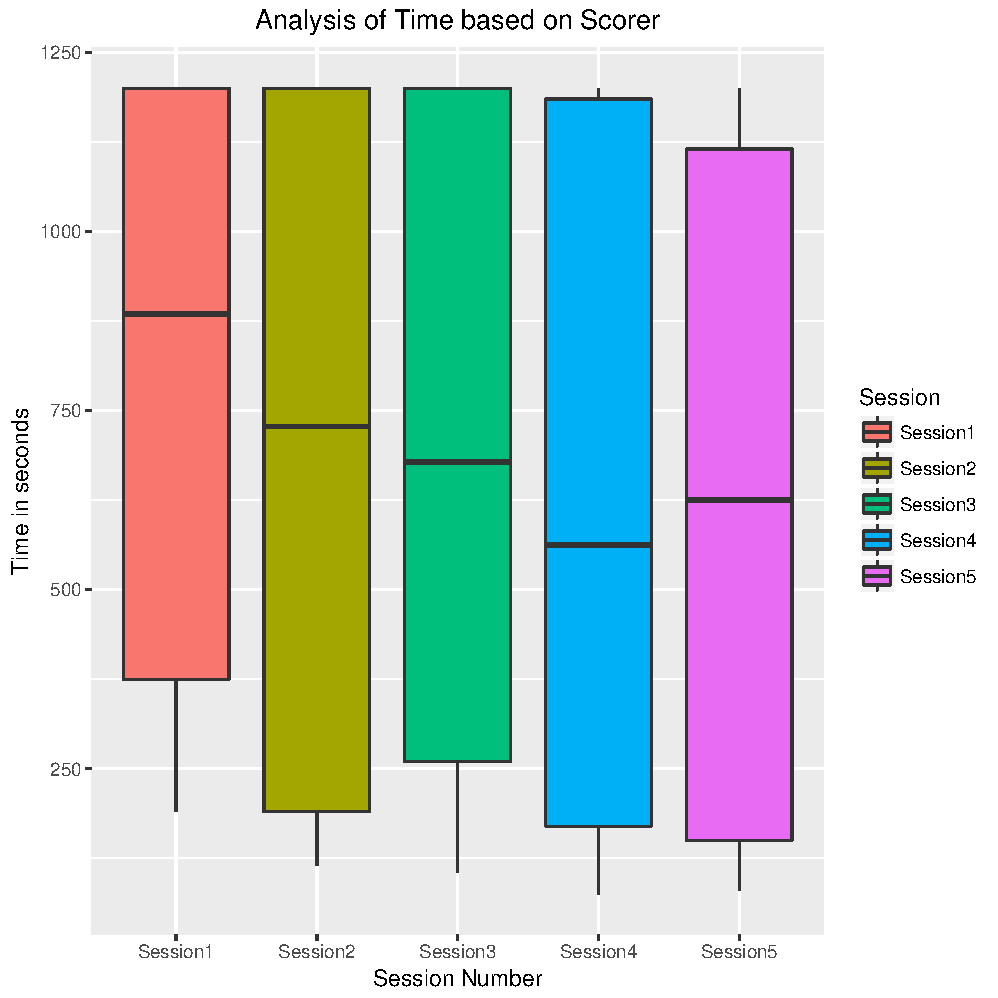
\includegraphics[width=\linewidth]{SessionVsTime.pdf}
	\caption{Analysis of Time based on Session}
	\end{minipage}
\end{figure}\\
\textbf{Inference}:\\
We observe that the means of Time vs Scorer or Gender do not have highly significant difference. Although, Task does have significant difference, we do not take it as a notifiable inference, because the time limits are different for each tasks, with time to complete suturing task being. 20 minutes. Hence, From the summary and the plots we infer that the time taken highly depends on the sessions.\\
\\
\FloatBarrier
\subsection*{3. Performance Analysis of Suturing Task}
\addcontentsline{toc}{subsection}{Performance Analysis of Suturing Task}
\textbf{Approach:Linear Model}:\\
\begin{figure}[!htb]
	\begin{minipage}[c]{0.5\linewidth}
	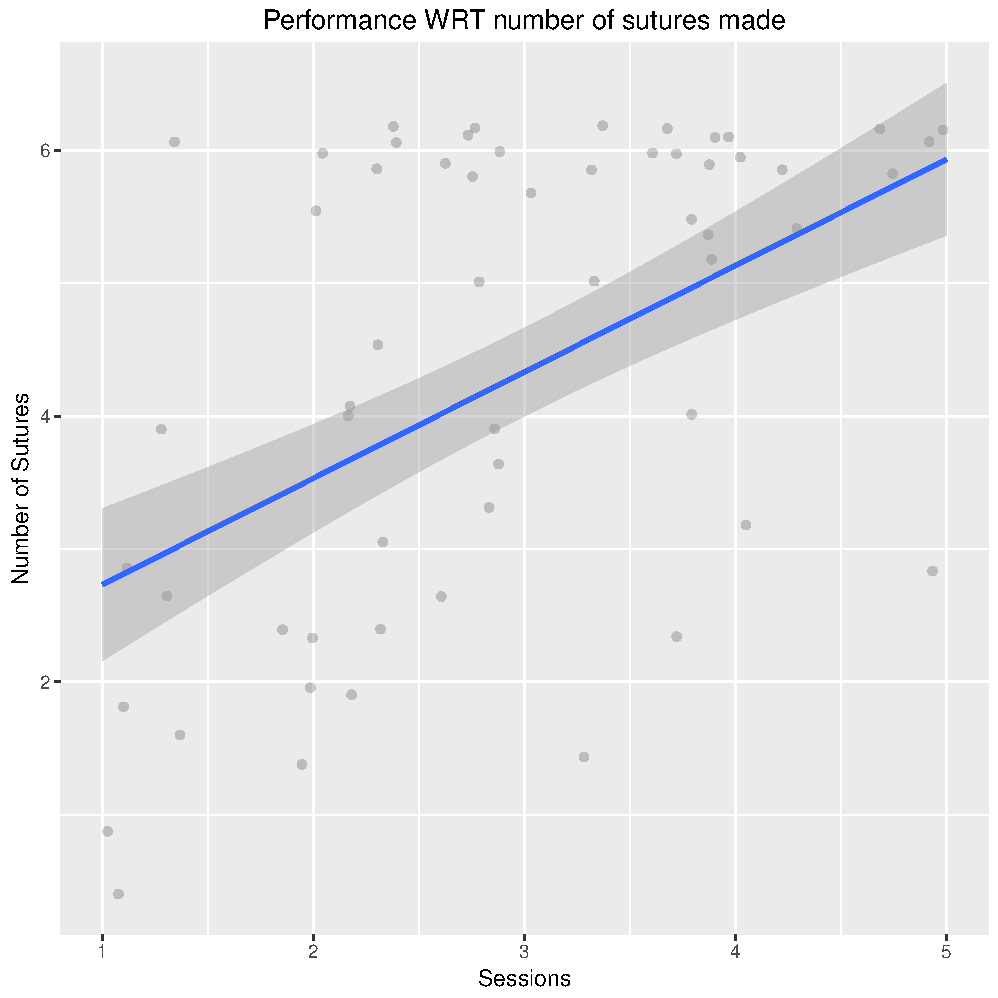
\includegraphics[width=\linewidth]{PerformanceWRTSutures.pdf}
	\caption{Performance WRT number of sutures made}
	\end{minipage}
	\hfill
	\begin{minipage}[c]{0.5\linewidth}
	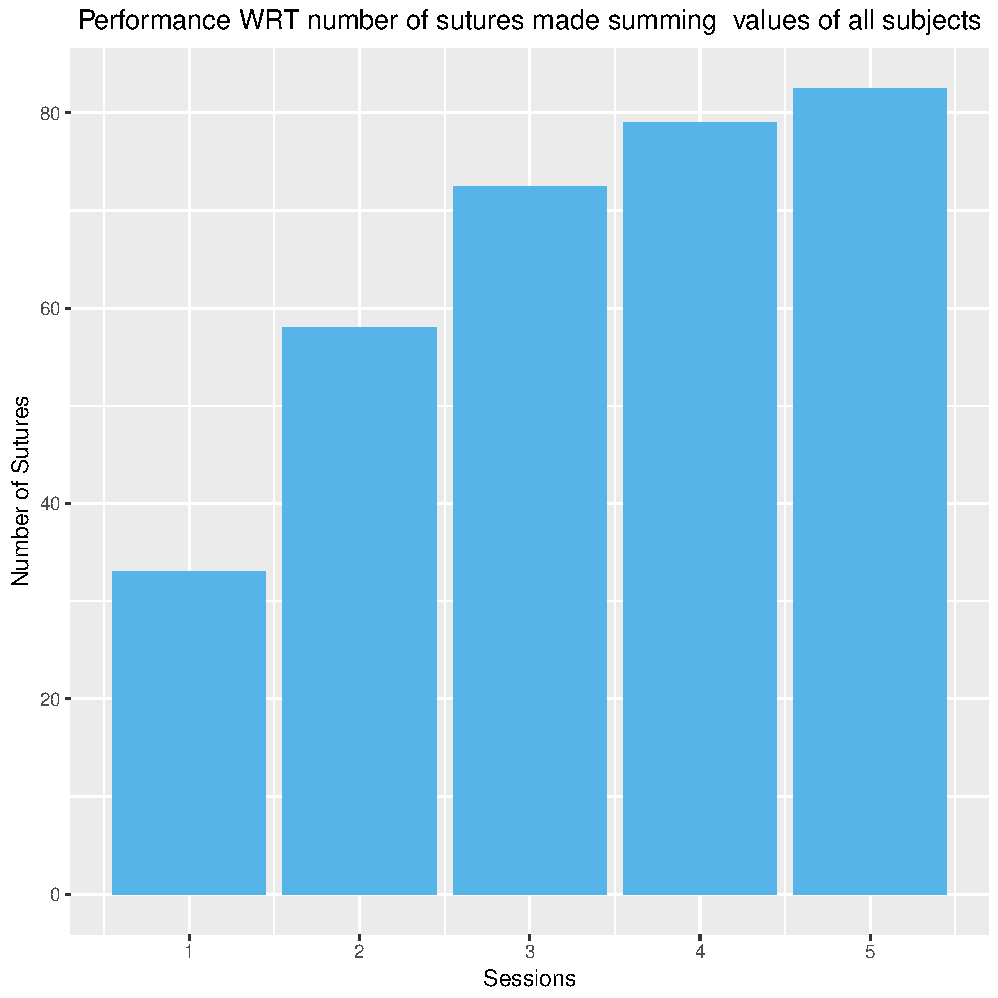
\includegraphics[width=\linewidth]{PerformanceWRTSutures_bar.pdf}
	\caption{Performance WRT number of sutures summed across all subjects}
	\end{minipage}
\end{figure}
\begin{figure}[!htb]
	\centering
	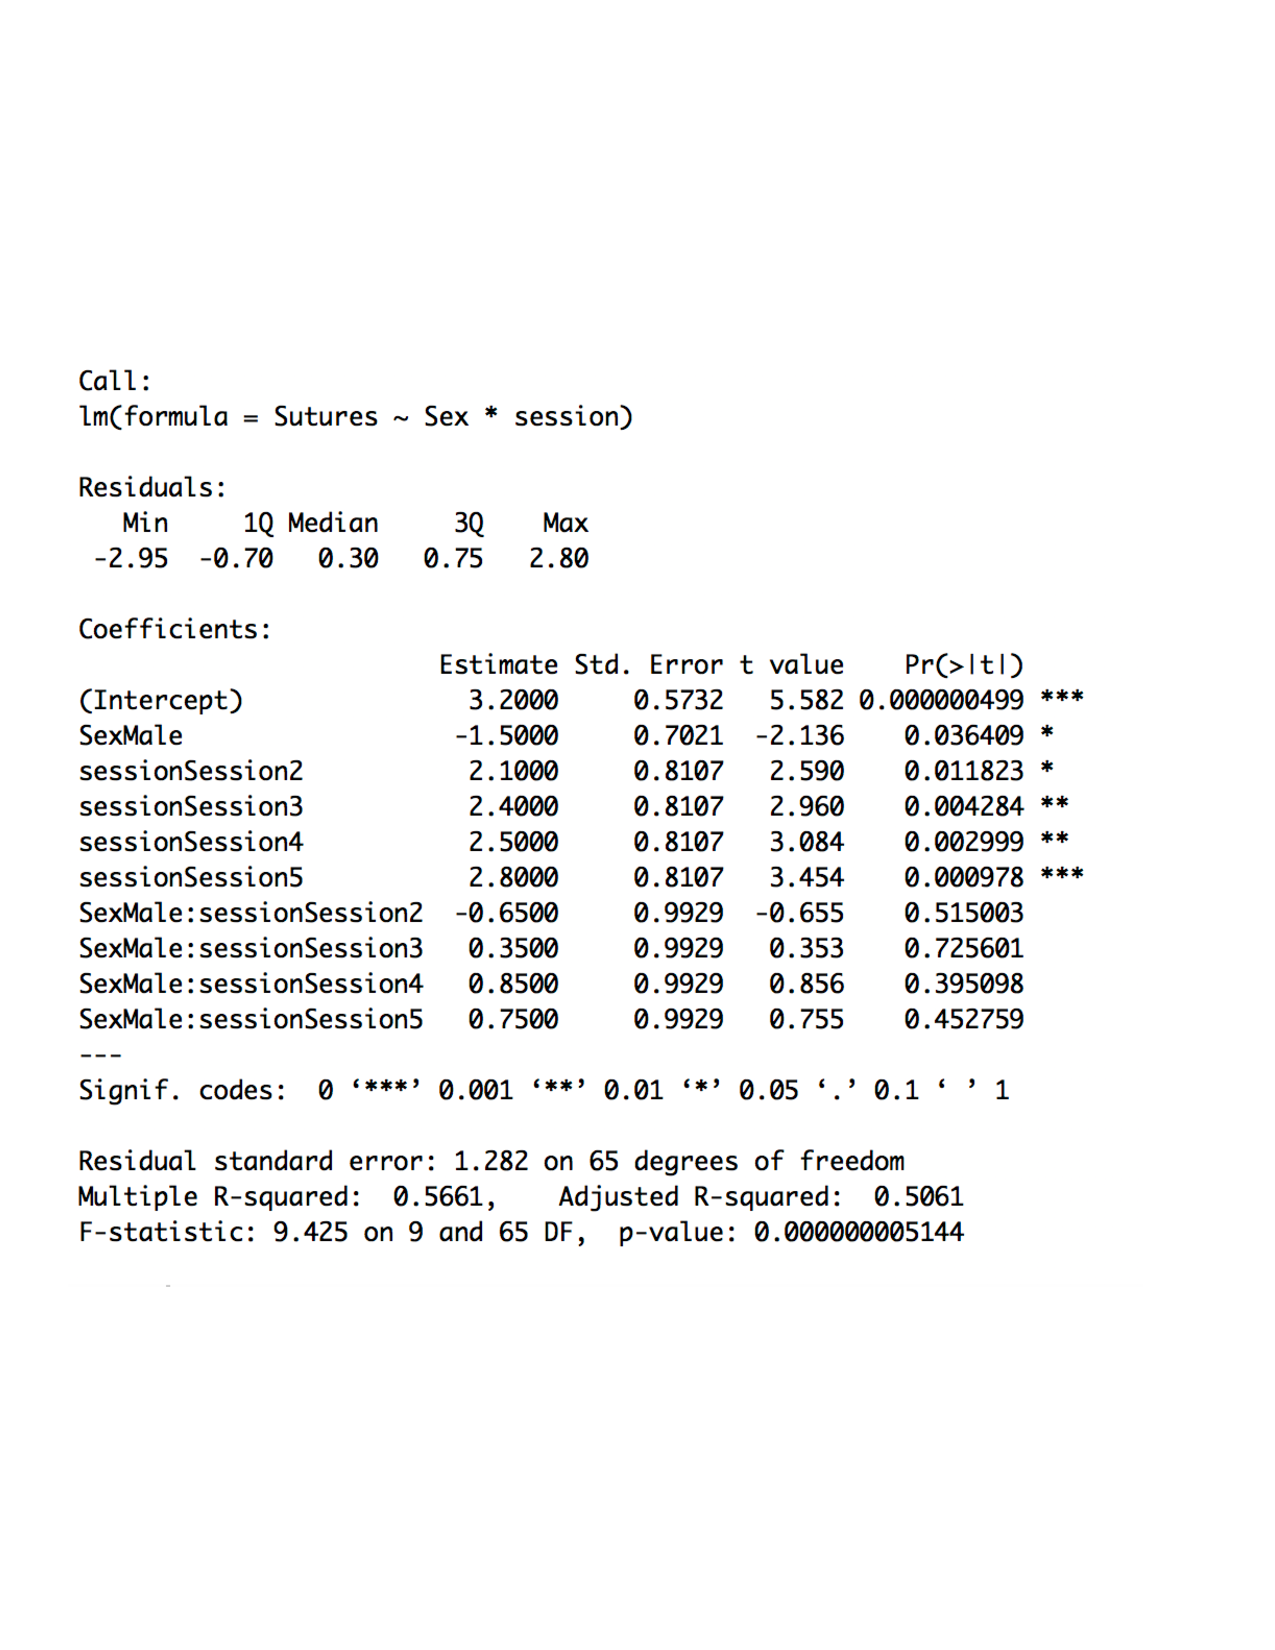
\includegraphics[width=0.5\textwidth]{Suture_Sex_Summary.pdf}
	\caption{Analysis of Linear Model}
	\centering
\end{figure}\\
\begin{figure}[!htb]
	\centering
	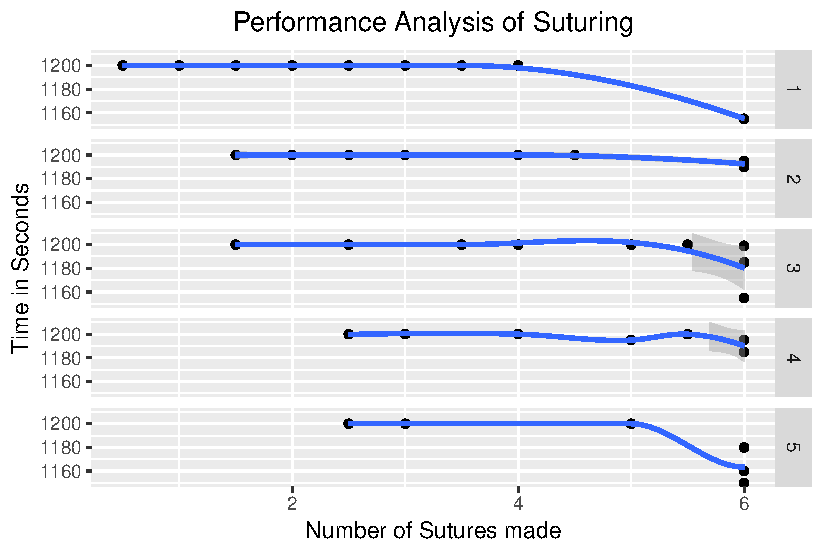
\includegraphics[width=0.5\textwidth]{SuturingVsTime.pdf}
	\caption{Performance Analysis of Suturing overTime }
	\centering
\end{figure}\\
From the figures, we understand that the number of sutures increases with each session. \\
To summarize it over all the subjects, we draw the bar plot with values of all subjects summed under each session , which gives us an understanding that with each session, the performance increases across all subjects.\\
When creating the linear model, and performing the analysis, we observe that the number of sutures is highly dependent on sessions .
Also, from the Performance analysis with respect to time plot(Figure:23), we infer that as the time decreases, the subjects are able to make more number of sutures and as number of session increases, the performance gets better.
\textbf{Inference}:\\
The number of sutures made increases with each session and takes less time, i.e the subjects are performing well.\\
\\
\FloatBarrier
\subsection*{4. Analysis of Scorers on Task:}
\addcontentsline{toc}{subsection} {Analysis of Scorers on Task}
\textbf{Hypothesis}:\\
$Null Hypothesis : H_0 = $ The mean of scores is same for both the Scorers\\
$Alternate Hypothesis : H_1 = $ The  mean of scores is different for both the Scorers\\
\\
\textbf{Approach:Wilcox Test}:\\
\begin{figure}[!htb]
	\begin{minipage}[c]{0.5\linewidth}
	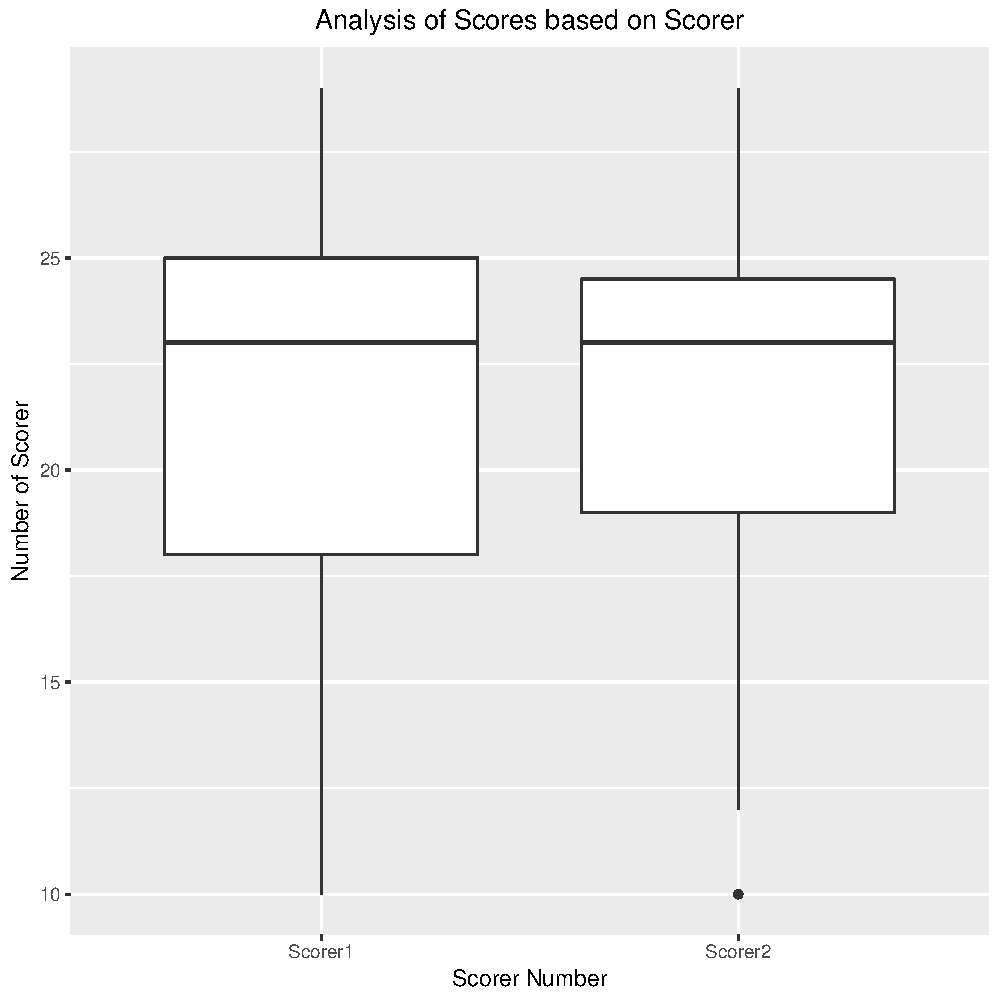
\includegraphics[width=\linewidth]{Cutting_ScorerVsScore.pdf}
	\caption{ Cutting Scores}
	\end{minipage}
	\hfill
	\begin{minipage}[c]{0.5\linewidth}
	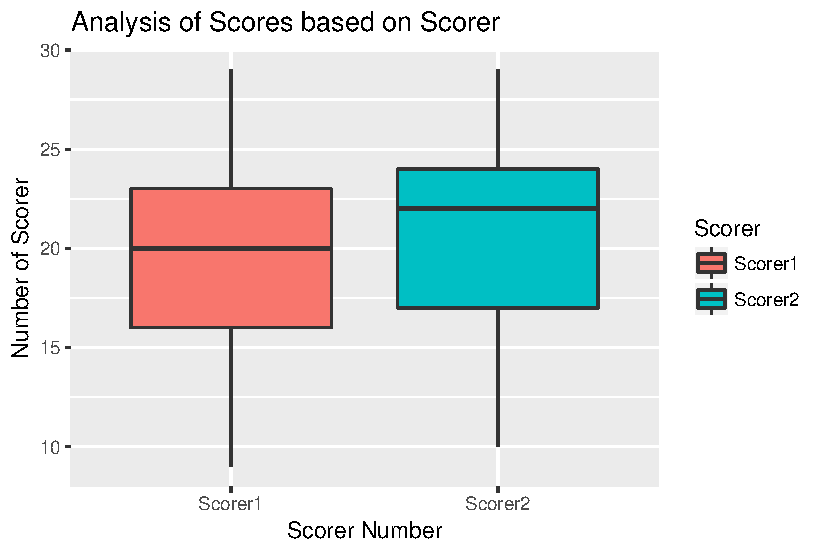
\includegraphics[width=\linewidth]{Suturing_ScorerVsScore.pdf}
	\caption{Suturing Scores}
	\end{minipage}
\end{figure}
\\
Cutting : When performed Wilcox test, p-value is greater than 0.05, which applies the means have not changed\\
Suturing: When performed Wilcox test, p-value is less than 0.05, which states that the means of the scorers is different. \\
\\
\textbf{Inference}:\\
Scorer has an effect for Suturing and Cutting\\
\FloatBarrier
\subsection*{5. Analysis of Number of Sutures made with respect to sex and sessions:}
\addcontentsline{toc}{subsection} {Analysis of Number of Sutures made wrt. sex and sessions}
\textbf{Hypothesis}:\\
$Null Hypothesis : H_0 = $ The number of sutures made is not significant on sex of the subject\\
$Alternate Hypothesis : H_1 = $ The number of sutures made is  significant on sex of the subject\\
\\
\begin{figure}[!htb]
	\centering
	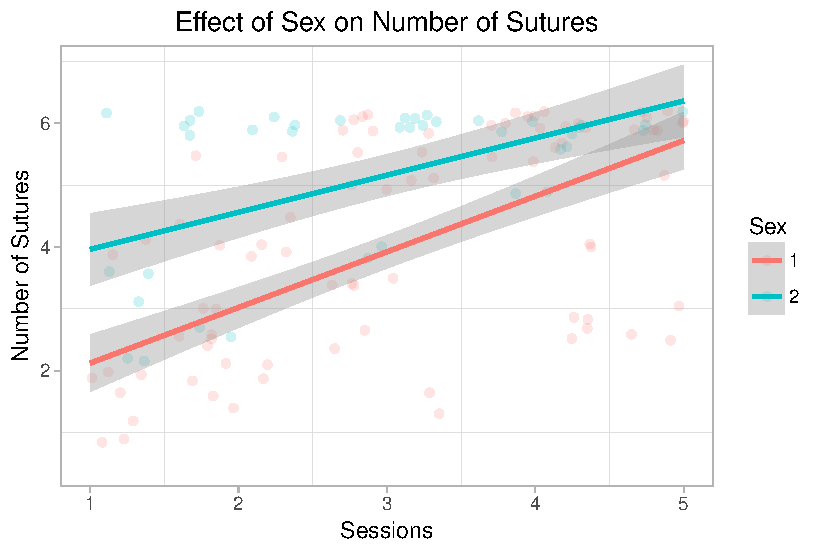
\includegraphics[width=0.5\textwidth]{SuturingVsSex.pdf}
	\caption{Interaction plot of Number of Sutures made wrt to Sex and Session}
	\centering
\end{figure}
\\
When performing the analysis for effect of Sutures on interaction of Sex and Sessions, we observe that, the p-value is 6.44e-11 which is way less than 0.05.\\
Also, from the interaction plot, we understand that the number of sutures made increases with the number of sessions and females make more number of sutures than males in average.\\
\\
\textbf{Inference}:\\
Sex has an effect on Number of Sutures made and females made more number of Sutures in 20 minutes and the number os sutures increases with each session, i.e subject's performance gets better with each session.\\






\newpage


\section*{Conclusion}
\addcontentsline{toc}{section}{Conclusion}



%-------------------------------------------------------------------------------
% Appendix
%-------------------------------------------------------------------------------
\newpage
\section*{Appendix}
\addcontentsline{toc}{section}{Appendix}
\subsection*{List of Figures}
\addcontentsline{toc}{subsection}{List of Figures}

%-------------------------------------------------------------------------------
% REFERENCES
%-------------------------------------------------------------------------------
\newpage
\section*{References}
\addcontentsline{toc}{section}{References}




\end{document}

